\documentclass[11pt, final, journal, twoside, a4paper]{IEEEtran}



% *** CITATION PACKAGES ***
%
%\usepackage{cite}


% *** MATH PACKAGES ***
%
\usepackage[cmex10]{amsmath}

\interdisplaylinepenalty=2500


% *** ALIGNMENT PACKAGES ***
%
\usepackage{array}

% *** FLOAT PACKAGES ***
%
\usepackage{fixltx2e}
\usepackage{float}

\usepackage{stfloats}


% *** PDF, URL AND HYPERLINK PACKAGES ***
%
\usepackage{url}
\usepackage[pdftex]{graphicx}
\usepackage{cite}

\usepackage[dutch]{babel}


\begin{document}

\graphicspath{ {Figures/} }
%
% paper title
% Titles are generally capitalized except for words such as a, an, and, as,
% at, but, by, for, in, nor, of, on, or, the, to and up, which are usually
% not capitalized unless they are the first or last word of the title.
% Linebreaks \\ can be used within to get better formatting as desired.
% Do not put math or special symbols in the title.
\title{Een Ziekte Inbedding leren met het gebruik van Veralgemeende Word2Vec Methoden}
%
%
% author names and IEEE memberships
% note positions of commas and nonbreaking spaces ( ~ ) LaTeX will not break
% a structure at a ~ so this keeps an author's name from being broken across
% two lines.
% use \thanks{} to gain access to the first footnote area
% a separate \thanks must be used for each paragraph as LaTeX2e's \thanks
% was not built to handle multiple paragraphs
%

\author{Milan van der Meer}% <-this % stops a space




% The paper headers
\markboth{}%
{\textbf{Een Ziekte Inbedding leren met het gebruik van Veralgemeende Word2Vec Methoden}}
% The only time the second header will appear is for the odd numbered pages
% after the title page when using the twoside option.
% 
% *** Note that you probably will NOT want to include the author's ***
% *** name in the headers of peer review papers.                   ***
% You can use \ifCLASSOPTIONpeerreview for conditional compilation here if
% you desire.



% make the title area
\maketitle

% As a general rule, do not put math, special symbols or citations
% in the abstract or keywords.
\begin{abstract}
In de medische wereld is er een stijgend gebruik van Electronic Health Records (EHRs). Hierdoor is er meer medische data beschikbaar en is er de mogelijkheid om nieuwe verbanden te vinden. Deze verbanden kunnen onderhanden gebruikt worden om de werking van medicaties te testen, kosten te bepalen van bepaalde ziektebeelden, en het vinden van nieuwe relaties tussen verschillende ziekten. \\
In dit nieuwe vakgebied van EHR analytics, is er een beperkt gebruik van recent machine learning technieken. Het doel van dit paper: het gebruiken van recente machine learning technieken om verbanden te vinden in EHRs.\\

Om dit te kunnen doen, maken we het verband tussen zinnen van woorden en sequenties van EHR events. Met de analogie introduceren wij veralgemeende Word2Vec methoden. Deze breiden we uit met DeepWalk voor performantie redenen aangezien dit ons toelaat om kleinere datasets te genereren. Vervolgens lossen we een Word2Vec probleem op namelijk het niet kunnen verwerken van ongeziene instanties. Hiervoor gebruiken we een k-nearest neighbors methode in combinatie met Word2Vec. \\

We testen $504$ verschillende parameter settings om onze modellen te bouwen. Deze modellen worden vervolgens getest en vergeleken met een paper over Deense EHRs. We vinden dat er een $60$\% match is tussen onze modellen en de Deense modellen. Hieruit concluderen we dat onze methodes belovend zijn zeker aangezien we verschillende benadering gebruiken die niet in de Deense EHRs aanwezig zijn. We concluderen ook dat doordat alle modellen hetzelfde scoren, de voorgestelde uitbreidingen op Word2Vec performant zijn.

\end{abstract}

% Note that keywords are not normally used for peerreview papers.
\begin{IEEEkeywords}
Inbedding, clustering, Word2Vec, EHR analytics
\end{IEEEkeywords}






% For peer review papers, you can put extra information on the cover
% page as needed:
% \ifCLASSOPTIONpeerreview
% \begin{center} \bfseries EDICS Category: 3-BBND \end{center}
% \fi
%
% For peerreview papers, this IEEEtran command inserts a page break and
% creates the second title. It will be ignored for other modes.
\IEEEpeerreviewmaketitle



\section{Electronic Health Records Analytics}

\IEEEPARstart{I}{n} de medische wereld is er een stijgend gebruik van medische hulp systemen. Deze systemen maken het mogelijk om medische data op een eenvoudige manier op te slaan. Voorbeelden hiervan zijn, dokters bezoeken, hospitalisatie, labo resultaten, en anderen, zie figuur \ref{fig:matrixPatient}. Deze gegevens worden samen opgeslagen in een Electronic Health Record (EHR) \cite{EHRworld:article}. \\

\begin{figure}[!htb]
	\centering
	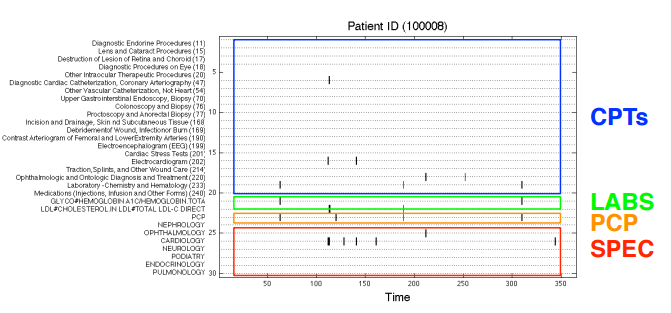
\includegraphics[width=2.5in]{matrixPatient.png}
	\caption{Example of an EHR transformed into a matrix structure \cite{EHRrecommender:article}}
	\label{fig:matrixPatient}
\end{figure}

Door deze stijging in beschikbare medische gegevens, zijn er verschillende partijen zoals dokters, hospitalen, en overheden met interesse om nieuwe verbanden te vinden hierin. Deze verbanden kunnen onderhanden gebruikt worden om de werking van medicaties te testen, kosten te bepalen van bepaalde ziektebeelden, en het vinden van nieuwe relaties tussen verschillende ziekten. \\
Omdat er vele problemen zijn rond EHRs zoals privacy, grote hoeveelheden data, complexe structuren, en verschillende gebruikte ziekte coden (bv. MedDRA \cite{MedDRA:online} of ICD-10 \cite{MedDRA:online}) , zijn er recent verschillende onderzoeksgroepen gevormd die zich focusen op de analyse van EHRs. Deze groepen gebruiken van eenvoudige methoden tot zeer complexe methoden zoals querying, statistische analyses, data mining, en machine learning algoritmes \cite{EHRbigdata:slides} \cite{EHRquery:journal} \cite{EHRrecommender:article} \cite{EHRmining:article}. \\

Voor dit artikel is een wel bepaald onderzoek zeer relevant namelijk het tot nu toe grootste EHR onderzoek \cite{Brunak:article}. Dit onderzoek is gedaan met behulp van een Deense dataset waarop men verschillende ziekte cluster zoekt met behulp van data mining methoden. Als resultaat hebben ze dus een overzicht van verschillende disease trajectory clusters, zie figuur \ref{fig:clusterGraphDanish}.

\begin{figure}[!htb]
	\centering
	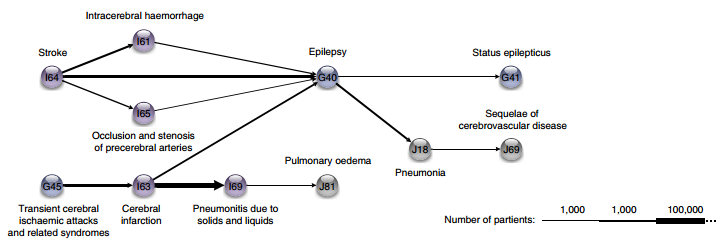
\includegraphics[width=2.5in]{clusterGraphDanish.png}
	\caption{Cerebrovascular disease trajectory cluster for the Danish population \cite{Brunak:article}}
	\label{fig:clusterGraphDanish}
\end{figure}
 
\hfill June 3, 2016



\section{Veralgemeende Word2Vec Methoden}
In deze sectie leggen we de analogie tussen zinnen van woorden en sequenties van EHR events. Door deze analogie, kunnen we de link leggen tussen Word2Vec \cite{w2vOriginal:article} en medische data.

\subsection{Data representatie}

De medische geschiedenis van een patient kan gezien worden als een tijdserie van EHR events. We noteren een EHR event als een vector $m^p_t$, met $p$ een patienten nummer en $t$ een tijdstip. Dit betekent dat elke patient een sequentie heeft van vectors, namelijk $s^p = m^p_t, m^p_{t+1}, m^p_{t+3}, \ldots$ Een vector kan waarden bevatten zoals bloeddruk, leeftijd, diagnose, en anderen (zie figuur \ref{fig:matrixPatient}).

\subsection{Veralgemeende Word2Vec}

Word2Vec wordt typisch toegepast op grote tekst corpusen. Met deze methode kan een inbedding worden gevonden waar woorden worden geprojecteerd naar een nieuwe vector ruimte. In deze vector ruimte worden de relaties tussen de woorden weergegeven door afstand tussen elkaar. \\

Een medische dataset kan worden beschouwd als een grote tekst corpus. Het bevat verschillende patienten (of zinnen) die elke een sequentie van EHR events hebben (of woorden). Met deze analogie, kunnen we Word2Vec toepassen op medische data. Op deze manier leren we een inbedding voor verschillende EHR events. \\
Andere soorten vergelijkingen zijn alreeds gemaakt zoals met protein sequenties \cite{protvec:article}.

\subsection{Knn Word2Vec}

Vervolgend lossen we een Word2Vec probleem op namelijk het kunnen verwerken van ongeziene instanties. Hiervoor gebruiken we een k-nearest neighbors methode \cite{knn:article} in combinatie met Word2Vec. \\

Deze knn methode kan toegepast worden omdat we aan het werken zijn met EHR events. Op basis van de EHR events die zich in de lookup table van het getrainde Word2Vec model bevinden, kunnen we de knn vinden voor een ongeziene EHR event. Op basis van deze knn EHR events, nemen we het gewogen gemiddelde van hun representaties in de nieuwe vector ruimte. Dit gewogen gemiddelde is de nieuwe vector representatie voor het ongeziene EHR event.

\subsection{Veralgemeende DeepWalk}

DeepWalk \cite{deepwalkMain:article} begint van een grafen-structuur en is daardoor niet direct toepasbaar op EHR data. Een voordeel van DeepWalk is dat het een methode aanbiedt om op basis van de originele dataset een kleinere dataset te maken. Dit doet het aan de hand van gewogen random walks. Met deze kleinere dataset, kunnen we een Word2Vec model sneller trainen. \\

Om deze random walks uit te kunnen voeren, moeten we eerst onze EHR data omzetten naar een grafen structuur. Dit doen we aan de hand van de sequenties in de originele dataset. Elke sequentie kan worden omgezet naar een directed graaf. Overeenkomstige vertices worden dan verbonden met elkaar en de gewichten van de edges worden aangepast op basis van de frequentie dat dezelfde vertices elkaar opvolgen.


\section{Resultaten}


\subsection{Parameters}


De performantie van een neuraal netwerk hangt sterk af van de gekozen waarden voor de parameters. Het tunen van deze parameters is een moeilijk probleem en complexe methoden zijn alreeds voorgesteld om dit op lossen \cite{tuning:article}. We kozen $504$ verschillende parameter settings om onze modellen te trainen. Merk op dat dit geen paper is over parameter tuning en daardoor het gebruik van de bovengenoemde methode mogelijk is in later werk. \\
In tabel \ref{tab:parameters}, zie je een overzicht van alle gekozen parameters. Alle mogelijke combinaties van deze parameters zijn getest. \\

\begin{table*}[!htb]
\centering

\begin{tabular}{llll}
\hline
Parameter                                    & Generalized Word2Vec  & Knn Word2Vec          & DeepWalk              \\ \hline
\multicolumn{1}{l|}{Vectorlength}            & {[}50, 100{]}         & {[}50, 100{]}         & {[}50, 100{]}         \\
\multicolumn{1}{l|}{Batch Size}              & 500                   & 500                   & 500                   \\
\multicolumn{1}{l|}{Epoch}                   & 1                     & 1                     & 1                     \\
\multicolumn{1}{l|}{Window Size}             & {[}5, 10, 15{]}       & {[}5, 10, 15{]}       & {[}5, 10, 15{]}       \\
\multicolumn{1}{l|}{Learning Rate}           & {[}0.025, 0.1{]}      & {[}0.025, 0.1{]}      & {[}0.025, 0.1{]}      \\
\multicolumn{1}{l|}{Minimum Word Freq} & {[}5, 10{]}           & {[}5, 10{]}           & {[}5, 10{]}           \\
\multicolumn{1}{l|}{ClusterK}                & {[}100, 1000, 5000{]} & {[}100, 1000, 5000{]} & {[}100, 1000, 5000{]} \\
\multicolumn{1}{l|}{K}                       & /                     & {[}10, 50, 100{]}     & /                     \\
\multicolumn{1}{l|}{Walklength}              & /                     & /                     & {[}5, 10, 15{]}      
\end{tabular}

\caption{De geteste parameters voor elke veralgemeende Word2Vec methode.}
\label{tab:parameters}
\end{table*}

Tot onze kennis, is er maar een enkele studie die zich toespitst op het tunen van Word2Vec parameters \cite{w2vTuning:article}. In deze studie nemen ze enkele random waarden en kijken vervolgens wat hun effecten zijn. Wij voeren een gelijkaardige methode uit door ook random waarden te nemen en kijken wat hun effecten zijn.

\subsection{Vergelijking Methoden}

We vergelijken onze $3$ methoden met elkaar op basis van de gemiddelde en maximum matching percentage. Voor elke methode gebruiken we de parameter setting die de hoogste waarde geeft voor de gemiddelde matching percentage. Deze settings kan je terugvinden in tabel \ref{tab:approaches}. \\

\begin{table*}[!htb]
\centering
\begin{tabular}{ccccccc}
\hline
Parameter                                   & \multicolumn{2}{c}{Generalized Word2Vec}         & \multicolumn{2}{c}{Knn Word2Vec}                 & \multicolumn{2}{c}{DeepWalk} \\ \hline
\multicolumn{1}{l|}{}                       & Exp 1 & \multicolumn{1}{c|}{Exp 2} & Exp 1 & \multicolumn{1}{c|}{Exp 2} & Exp 1  & Exp 2 \\ \hline
\multicolumn{1}{l|}{Vectorlength}           & 100          & \multicolumn{1}{c|}{50}           & 100          & \multicolumn{1}{c|}{50}           & 50            & 100          \\
\multicolumn{1}{l|}{Window Size}            & 15           & \multicolumn{1}{c|}{15}           & 5            & \multicolumn{1}{c|}{5}            & 5             & 10           \\
\multicolumn{1}{l|}{Learning Rate}          & 0.025        & \multicolumn{1}{c|}{0.025}        & 0.025        & \multicolumn{1}{c|}{0.025}        & 0.025         & 0.025        \\
\multicolumn{1}{l|}{Minimum Word Freq} & 10           & \multicolumn{1}{c|}{5}            & 5            & \multicolumn{1}{c|}{5}            & 10            & 5            \\
\multicolumn{1}{l|}{ClusterK}               & 100          & \multicolumn{1}{c|}{5000}         & 100          & \multicolumn{1}{c|}{5000}         & 100           & 5000         \\
\multicolumn{1}{l|}{K}                      & /            & \multicolumn{1}{c|}{/}            & 100          & \multicolumn{1}{c|}{100}          & /             & /            \\ 
\multicolumn{1}{l|}{Walklength}             & /            & \multicolumn{1}{c|}{/}            & /            & \multicolumn{1}{c|}{/}            & 5             & 15           \\ \hline
\multicolumn{1}{l|}{Average Matching \%}    & 29           & \multicolumn{1}{c|}{62}           & 33           & \multicolumn{1}{c|}{61}           & 27            & 61           \\
\multicolumn{1}{l|}{Maximum Matching \%}    & 56           & \multicolumn{1}{c|}{69}           & 69           & \multicolumn{1}{c|}{69}           & 61            & 69          
\end{tabular}

\caption{Best gevonden parameter setting voor elke methode.}
\label{tab:approaches}
\end{table*}

Elke methode heeft een gelijkaardige matching percentage, zeker als je kijkt naar het maximum matching percentage. We concluderen dat beide onze knn Word2Vec en DeepWalk dezelfde performantie hebben dan de basis veralgemeende Word2Vec. Dit betekent dat we nu ongeziene EHR events aankunnen met behulp van onze knn Word2Vec en ook dat we kleinere dataset kunnen gebruiken met behulp van DeepWalk zonder performantie te verliezen. \\

Het blijft moeilijk om te quantificeren hoe goed een match percentage van $60$\% is. Maar we maken de assumptie dat dit goed genoeg is om het potentieel van onze methoden aan te tonen. Zeker indien we rekening houden met de gebruikte benaderings methoden zoals de code mapping, verschillende datasets, en de categorizatie.

\section{Conclusie}

In dit paper legde we het nieuwe vakgebied rond EHR analytics uit en waarom het interessant is om verbanden tussen vershillende ziekten te vinden hierin. Onderzoeksgroepen gebruiken hiervoor allerhande methoden maar een beperkt aantal machine learning methoden worden gebruikt. \\

Daardoor stelden wij onze veralgemeende Word2Vec methoden voor zodat Word2Vec kan worden toegepast op medische data. Deze breiden we uit met DeepWalk voor performantie redenen aangezien dit ons toelaat om kleinere datasets te genereren. Vervolgend lossen we een Word2Vec probleem op namelijk het kunnen verwerken van ongeziene instanties. Hiervoor gebruiken we een k-nearest neighbors methode in combinatie met Word2Vec. \\

We hebben $504$ verschillende parameter settings getest om onze modellen te bouwen. Van deze parameter settings nemen wij diegene die voor elke model de hoogste gemiddelde matching percentage geeft tussen de Word2Vec clusters en de Deense clusters. \\

We vinden dat er een $60$\% match is tussen onze clusters en de Deense clusters. Hieruit concluderen we dat onze methodes belovend zijn zeker aangezien we verschillende benadering gebruiken die niet in de Deense EHRs aanwezig zijn. \\
We concluderen ook dat doordat alle modellen hetzelfde scoren, de voorgestelde uitbreidingen op Word2Vec performant zijn.

\section{Toekomstig Werk}

Een Word2Vec model kan gebruikt worden in combinatie met een neuraal netwerk. Dit neuraal netwerk maakt gebruik van de nieuwe vector representie om zijn voorspellingen te verbeteren. In de toekomst, zou het interessant zijn om ziektes van patienten te kunnen voorspellen hiermee en vervolgens te testen of het gebruik van onze Word2Vec methoden deze voorspellingen accurater maken. 


% An example of a double column floating figure using two subfigures.
% (The subfig.sty package must be loaded for this to work.)
% The subfigure \label commands are set within each subfloat command,
% and the \label for the overall figure must come after \caption.
% \hfil is used as a separator to get equal spacing.
% Watch out that the combined width of all the subfigures on a 
% line do not exceed the text width or a line break will occur.
%
%\begin{figure*}[!t]
%\centering
%\subfloat[Case I]{\includegraphics[width=2.5in]{box}%
%\label{fig_first_case}}
%\hfil
%\subfloat[Case II]{\includegraphics[width=2.5in]{box}%
%\label{fig_second_case}}
%\caption{Simulation results for the network.}
%\label{fig_sim}
%\end{figure*}
%
% Note that often IEEE papers with subfigures do not employ subfigure
% captions (using the optional argument to \subfloat[]), but instead will
% reference/describe all of them (a), (b), etc., within the main caption.
% Be aware that for subfig.sty to generate the (a), (b), etc., subfigure
% labels, the optional argument to \subfloat must be present. If a
% subcaption is not desired, just leave its contents blank,
% e.g., \subfloat[].


% An example of a floating table. Note that, for IEEE style tables, the
% \caption command should come BEFORE the table and, given that table
% captions serve much like titles, are usually capitalized except for words
% such as a, an, and, as, at, but, by, for, in, nor, of, on, or, the, to
% and up, which are usually not capitalized unless they are the first or
% last word of the caption. Table text will default to \footnotesize as
% IEEE normally uses this smaller font for tables.
% The \label must come after \caption as always.
%
%\begin{table}[!t]
%% increase table row spacing, adjust to taste
%\renewcommand{\arraystretch}{1.3}
% if using array.sty, it might be a good idea to tweak the value of
% \extrarowheight as needed to properly center the text within the cells
%\caption{An Example of a Table}
%\label{table_example}
%\centering
%% Some packages, such as MDW tools, offer better commands for making tables
%% than the plain LaTeX2e tabular which is used here.
%\begin{tabular}{|c||c|}
%\hline
%One & Two\\
%\hline
%Three & Four\\
%\hline
%\end{tabular}
%\end{table}


% Note that the IEEE does not put floats in the very first column
% - or typically anywhere on the first page for that matter. Also,
% in-text middle ("here") positioning is typically not used, but it
% is allowed and encouraged for Computer Society conferences (but
% not Computer Society journals). Most IEEE journals/conferences use
% top floats exclusively. 
% Note that, LaTeX2e, unlike IEEE journals/conferences, places
% footnotes above bottom floats. This can be corrected via the
% \fnbelowfloat command of the stfloats package.





% Can use something like this to put references on a page
% by themselves when using endfloat and the captionsoff option.
\ifCLASSOPTIONcaptionsoff
  \newpage
\fi



% trigger a \newpage just before the given reference
% number - used to balance the columns on the last page
% adjust value as needed - may need to be readjusted if
% the document is modified later
%\IEEEtriggeratref{8}
% The "triggered" command can be changed if desired:
%\IEEEtriggercmd{\enlargethispage{-5in}}

% references section
%\bibliographystyle{IEEEtran}
\begin{thebibliography}{10}

\bibitem{MedDRA:online}
{MedDRA}.
\newblock \url{http://www.meddra.org/}.
\newblock (Accessed on 05/03/2016).

\bibitem{w2vNgram:online}
{The Speech Recognition Wiki}.
\newblock \url{http://recognize-speech.com/}.
\newblock (Accessed on 05/16/2016).


\bibitem{WHO_ICD:online}
{WHO | International Classification of Diseases (ICD)}.
\newblock \url{http://www.who.int/classifications/icd/en/}.
\newblock (Accessed on 04/27/2016).

\bibitem{protvec:article}
E.~Asgari and M.~R.~K. Mofrad.
\newblock {Continuous Distributed Representation of Biological Sequences for
  Deep Proteomics and Genomics}.
\newblock {\em PLoS ONE}, 10(11):1--15, 11 2015.

\bibitem{tuning:article}
M.~Bashiri and A.~F. Geranmayeh.
\newblock {Tuning the parameters of an artificial neural network using central
  composite design and genetic algorithm}.
\newblock {\em Scientia Iranica}, 18(6):1600 -- 1608, 2011.

\bibitem{EHRmining:article}
C.~Bennett and T.~Doub.
\newblock {Data Mining and Electronic Health Records: Selecting Optimal
  Clinical Treatments in Practice}.
\newblock {\em CoRR}, abs/1112.1668, 2011.

\bibitem{knn:article}
T.~M. Cover.
\newblock {Nearest neighbor pattern classification}.
\newblock 1982.

\bibitem{w2vReason1:online}
{Google Brain Team}.
\newblock {Vector Representations of Words}.
\newblock
  \url{https://www.tensorflow.org/versions/0.6.0/tutorials/word2vec/index.html}.
\newblock (Accessed on 05/16/2016).

\bibitem{w2vNgram:article}
D.~Guthrie, B.~Allison, W.~Liu, L.~Guthrie, and Y.~Wilks.
\newblock {A Closer Look at Skip-gram Modelling}.

\bibitem{EHRquery:journal}
A.~Hameurlain, J.~Kung, R.~Wagner, H.~Decker, L.~Lhotska, and S.~Link, editors.
\newblock {\em {Transactions on Large-Scale Data- and Knowledge-Centered
  Systems {IV} - Special Issue on Database Systems for Biomedical
  Applications}}, volume 8980 of {\em Lecture Notes in Computer Science}.
  Springer, 2011.

\bibitem{Brunak:article}
A.~B. Jensen, P.~L. Moseley, T.~I. Oprea, S.~G. Ellesoe, R.~Eriksson,
  H.~Schmock, P.~B. Jensen, L.~J. Jensen, and S.~Brunak.
\newblock {Temporal disease trajectories condensed from population-wide
  registry data covering 6.2 million patients}.
\newblock {\em Nat Commun}, 5, Jun 2014.
\newblock Article.

\bibitem{EHRbigdata:slides}
C.~K.~R. Jimeng~Sun.
\newblock {Big Data Analytics for Healthcare}.
\newblock 2013.


\bibitem{w2vTuning:article}
O.~Levy, Y.~Goldberg, and I.~Dagan.
\newblock {Improving Distributional Similarity with Lessons Learned from Word
  Embeddings}.
\newblock {\em {TACL}}, 3:211--225, 2015.

\bibitem{w2vOriginal:article}
T.~Mikolov, I.~Sutskever, K.~Chen, G.~Corrado, and J.~Dean.
\newblock {Distributed Representations of Words and Phrases and their
  Compositionality}.
\newblock {\em CoRR}, abs/1310.4546, 2013.

\bibitem{OSIM:online}
{Observational Medical Outcomes Partnership}.
\newblock {OSIM2 - Observational Medical Dataset Simulator Generation 2 |
  Observational Medical Outcomes Partnership}.
\newblock \url{http://omop.org/OSIM2}.
\newblock (Accessed on 05/28/2016).

\bibitem{w2vNN:online}
C.~Olah.
\newblock {Deep Learning, NLP, and Representations - colah's blog}.
\newblock \url{http://colah.github.io/posts/2014-07-NLP-RNNs-Representations/}.
\newblock (Accessed on 05/16/2016).

\bibitem{deepwalkMain:article}
B.~Perozzi, R.~Al{-}Rfou, and S.~Skiena.
\newblock {DeepWalk: Online Learning of Social Representations}.
\newblock {\em CoRR}, abs/1403.6652, 2014.

\bibitem{w2vModels:article}
X.~Rong.
\newblock {word2vec Parameter Learning Explained}.
\newblock {\em CoRR}, abs/1411.2738, 2014.



\bibitem{EHRworld:article}
C.~P. Stone.
\newblock {A Glimpse at EHR Implementation Around the World: The Lessons the US
  Can Learn}.
\newblock 2014.

\bibitem{EHRsimilarity:article}
J.~Sun, F.~Wang, J.~Hu, and S.~Edabollahi.
\newblock {Supervised Patient Similarity Measure of Heterogeneous Patient
  Records}.
\newblock {\em SIGKDD Explor. Newsl.}, 14(1):16--24, Dec. 2012.

\bibitem{EHRrecommender:article}
F.~Wang, N.~Lee, J.~Hu, J.~Sun, and S.~Ebadollahi.
\newblock {Towards Heterogeneous Temporal Clinical Event Pattern Discovery: A
  Convolutional Approach}.
\newblock In {\em Proceedings of the 18th ACM SIGKDD International Conference
  on Knowledge Discovery and Data Mining}, KDD '12, pages 453--461, New York,
  NY, USA, 2012. ACM.

\end{thebibliography}






% that's all folks
\end{document}